\documentclass[a4paper,11pt]{article}
\usepackage{commonpackages}

\usepackage{listingsutf8}
\lstset{language=TeX, backgroundcolor=\color{mybackcolor}, frame=single, numbersep=5pt, belowcaptionskip=1\baselineskip, breaklines=true, basicstyle=\ttfamily}

\begin{document}
\title{Mode d'emploi des balises personnalisées}
\date{}
\maketitle

Afin de pouvoir ajouter des vidéos Youtube, une fenêtre Geogebra, des images, du code source et des
solutions, des balises personnalisées peuvent être ajoutées au document LaTeX. Voici leur fonctionnement.

\section{Vidéos Youtube}
Pour ajouter une vidéo Youtube, il suffit de connaître sa référence et d’utiliser la balise vidéo.\par

Code LaTeX:
\begin{lstlisting}
\video{U98Tk89SJ5M}
\end{lstlisting}

Rendu Web:\par
\video{U98Tk89SJ5M}

Par défaut, la taille de la fenêtre de la vidéo est 50\% de la largeur du texte. Il est possible de
changer la dimension en ajoutant un paramètre optionnel, celui-ci doit être noté entre crochets
et avant la référence de la vidéo.\par

Code LaTeX:
\begin{lstlisting}
\video[100]{U98Tk89SJ5M}
\end{lstlisting}

Rendu Web:\par
\video[100]{U98Tk89SJ5M}

Les vidéos peuvent être visionnées en plein écran.

\section{Fenêtre Geogebra}
Pour ajouter une fenêtre Geogebra, il faut tout d’abord créer le document Geogebra et le sauvegarder en ligne sur \href{https://www.geogebra.org/}{site de Geogebra}. Ensuite, il pourra être intégré au document LaTeX au moyen de la balise Geogebra.\par

Code LaTeX:
\begin{lstlisting}
\geogebra{esdhdhzd}
\end{lstlisting}

Rendu Web:\par
\geogebra{esdhdhzd}

Par défaut, la taille de la fenêtre Geogebra est 100\% de la largeur du texte, afin d’optimiser l’utilisation pour l’élève. Il est possible de changer la dimension en ajoutant un paramètre optionnel, celui-ci doit être noté entre crochets et avant la référence du document Geogebra.\par

Code LaTeX:
\begin{lstlisting}
\geogebra[75]{jdqu43nr}
\end{lstlisting}

Rendu Web:\par
\geogebra[75]{jdqu43nr}

Geogebra peut aussi être utilisé en plein écran.

\section{Image}
L’ajout d’images ne nécessite pas la création d’une balise personnalisée, toutefois pour que l’affichage soit correct au moment de la génération du HTML, il est nécessaire de définir les dimensions de celle-ci en fonction de la largeur du texte.\par

Code LaTeX:
\begin{lstlisting}
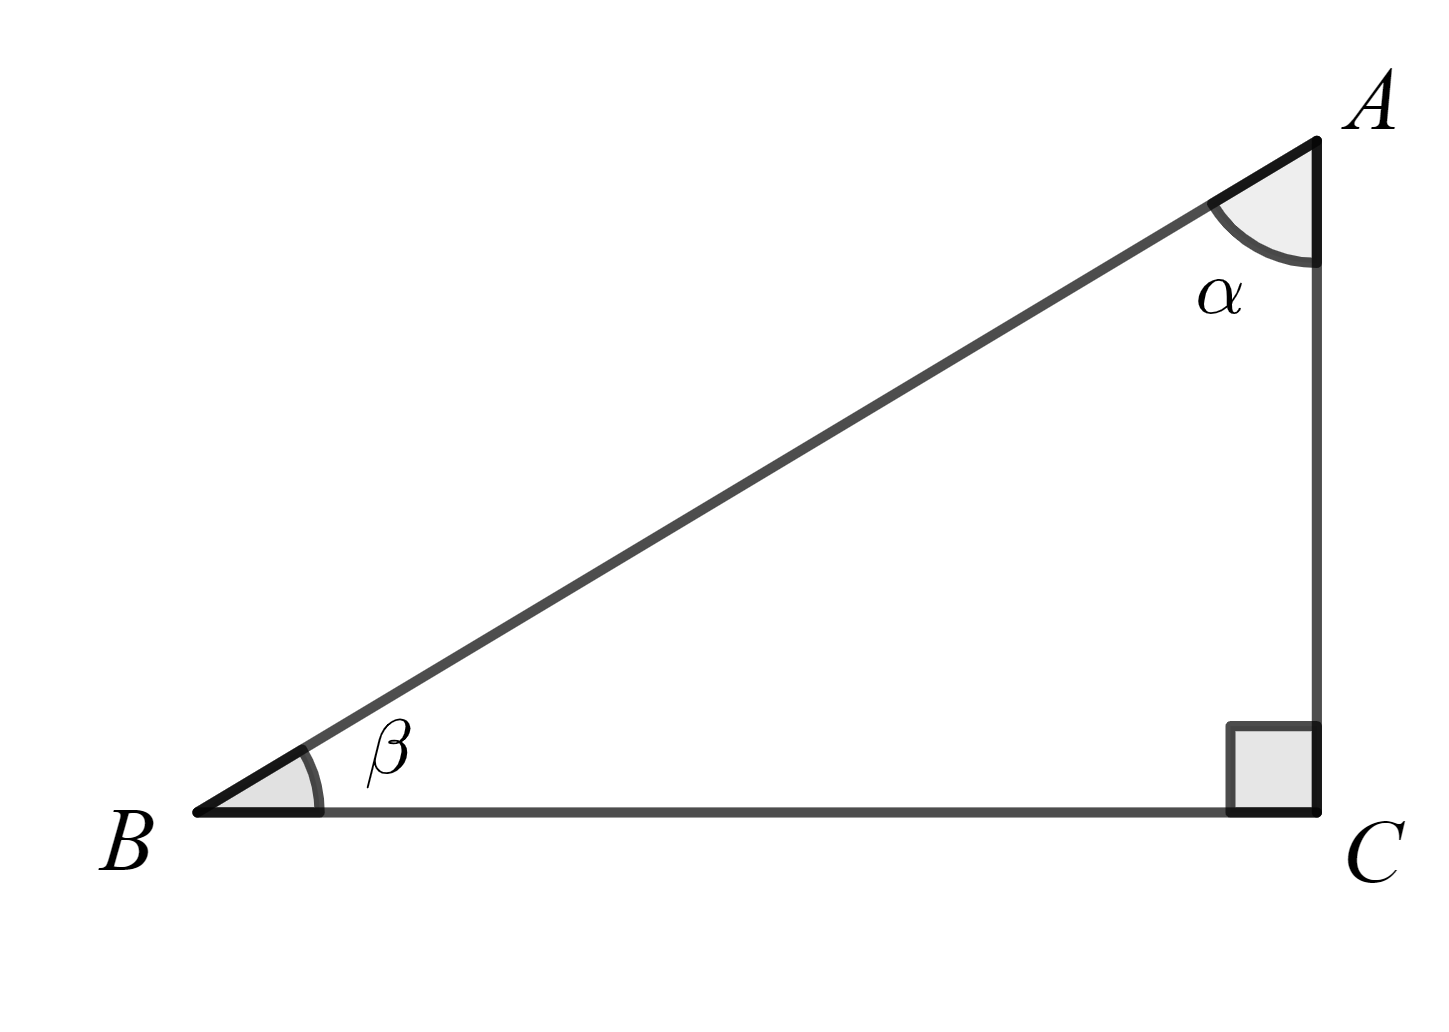
\includegraphics[width=0.5\textwidth]{images/pythagore.png}
\end{lstlisting}

Rendu Web:\par
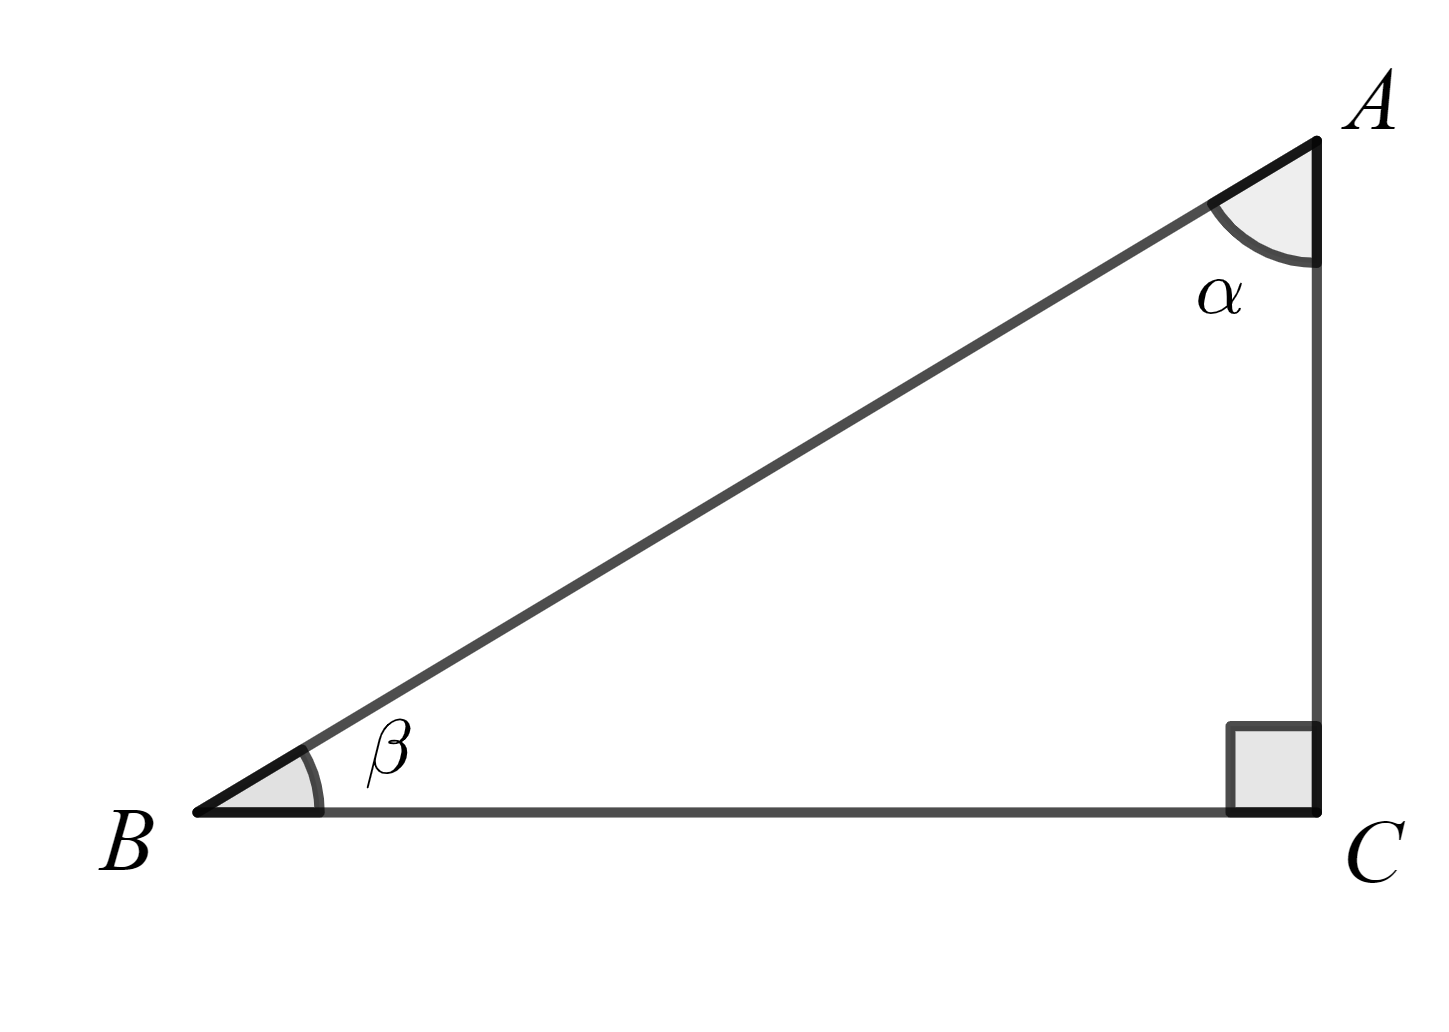
\includegraphics[width=0.5\textwidth]{images/pythagore.png}

\section{Code source}
\subsection{Code surligné}
Pour afficher du code source, celui-ci sera simplement inclus dans un environnement code. Afin que le surlignement se fasse correctement, il est obligatoire de définir le langage comme paramètre, par exemple python, html, css.\par

Code LaTeX:
\begin{lstlisting}
\begin{code}{python}
for i in range(10):
    print(i)
\end{code}
\end{lstlisting}

Rendu Web:\par
\begin{code}{python}
for i in range(10):
    print(i)
\end{code}

Le code est affiché avec une numérotation des lignes et surligné grâce à highlight.js.

\subsection{Code exécutable}
Actuellement, seul le langage Python peut être exécuté dans le navigateur. Pour cela, il faut ajouter le paramètre optionnel ”interactive”. En cliquant sur le bouton "Exécuter", le résultat s'affiche.\par

Code LaTeX:
\begin{lstlisting}
\begin{code}[interactive]{python}
t = float(input("Quelle température fait-il? "))
if t < 0:
    print("Ça gèle!")
elif t < 15:
    print("Il fait pas chaud!")
elif t < 25:
    print("Température idéale!")
else:
    print("Il fait trop chaud!")
\end{code}
\end{lstlisting}

Rendu Web:\par
\begin{code}[interactive]{python}
t = float(input("Quelle température fait-il? "))
if t < 0:
    print("Ça gèle!")
elif t < 15:
    print("Il fait pas chaud!")
elif t < 25:
    print("Température idéale!")
else:
    print("Il fait trop chaud!")
\end{code}

\subsection{Code source avec le module Turtle}
L’affichage de code contenant le module Turtle est fait dans un environnement graphique, il est
donc nécessaire de spécifier, quand il est utilisé. Cela se fait au moyen du paramètre optionnel
”interactive_turtle”.\par

Code LaTeX:
\begin{lstlisting}
\begin{code}[interactive_turtle]{python}
from turtle import *
from random import randint

penup()
goto(-100, -100)
pendown()
nb_cote_max = int(input("Combien de côtés voulez-vous au maximum? "))
colormode(255)
pensize(3)
for i in range(3, nb_cote_max + 1):
    for j in range(i):
        forward(100)
        left(360/i)
    pencolor(randint(0,255), randint(0, 255), randint(0,255))
\end{code}
\end{lstlisting}

Rendu Web:\par
\begin{code}[interactive_turtle]{python}
from turtle import *
from random import randint

penup()
goto(-100, -100)
pendown()
nb_cote_max = int(input("Combien de côtés voulez-vous au maximum? "))
colormode(255)
pensize(3)
for i in range(3, nb_cote_max + 1):
    for j in range(i):
        forward(100)
        left(360/i)
    pencolor(randint(0,255), randint(0, 255), randint(0,255))
\end{code}

\section{Solution}
Afin de pouvoir afficher ou non la solution des exercices, celle-ci sera inclue dans un environnement solution.\par

Code LaTeX:
\begin{lstlisting}
Dans un triangle rectangle en $C$, nous connaissons $\alpha=27^{\circ}$ et $c=8\,cm$. Résoudre ce triangle.

\begin{solution}
\begin{center}
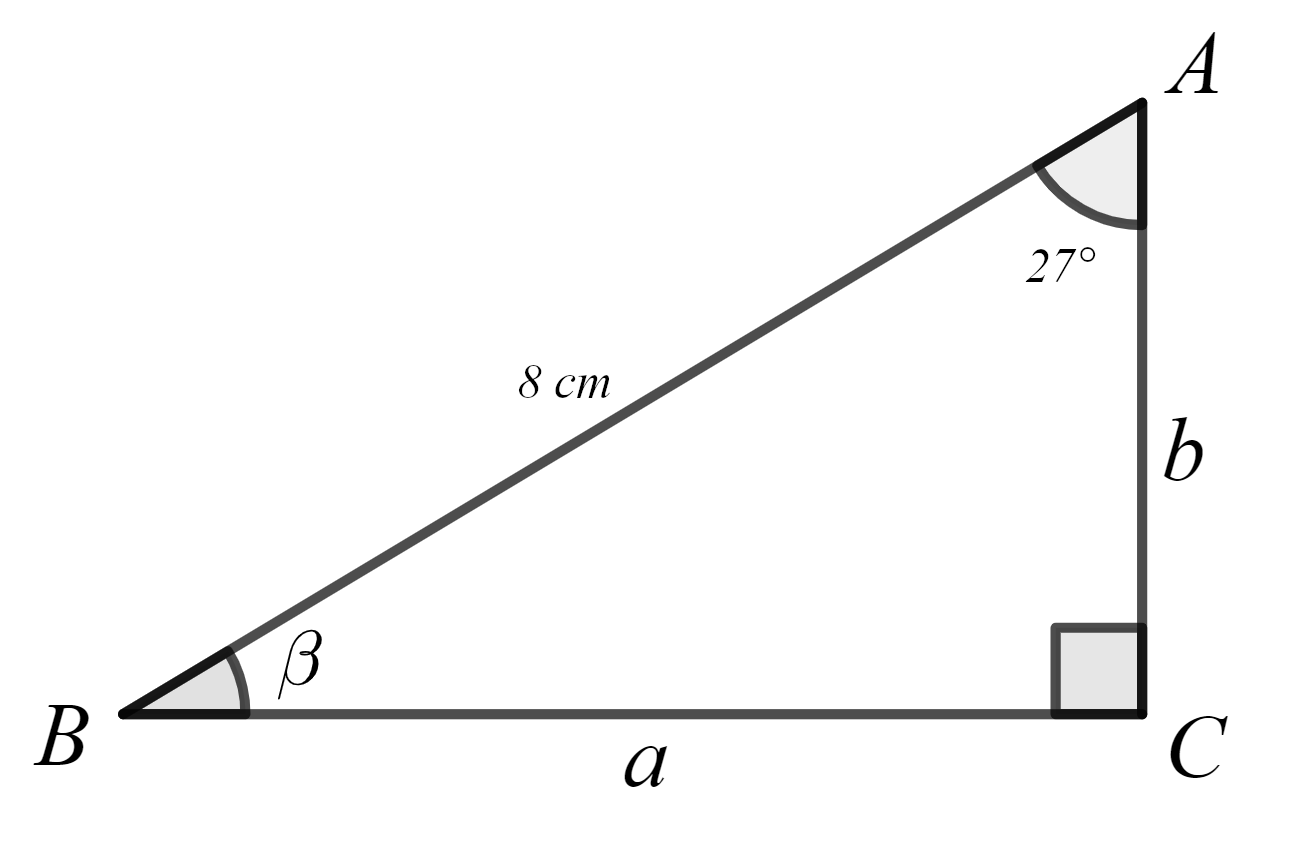
\includegraphics[width=1\textwidth]{images/trianglerectexemple.png}\\
\end{center}
$\beta=180-90-27=63^{\circ}$\\
En utilisant la trigonométrie:\\
$\sin(\alpha)=\dfrac{\text{opp}}{\text{hyp}} \Rightarrow \sin(27^{\circ})=\dfrac{\overline{BC}}{8}$\\
$\Rightarrow \overline{BC}=8 \cdot \sin(27^{\circ})=3.63\,cm$\\
$\cos(\alpha)=\dfrac{\text{adj}}{\text{hyp}} \Rightarrow \cos(27^{\circ})=\dfrac{\overline{AC}}{8}$\\
$\Rightarrow \overline{AC}=8 \cdot \cos(27^{\circ})=7.13\,cm$\\
\end{solution}
\end{lstlisting}

Rendu Web:\par
Dans un triangle rectangle en $C$, nous connaissons $\alpha=27^{\circ}$ et $c=8\,cm$. Résoudre ce triangle.\par

\begin{solution}
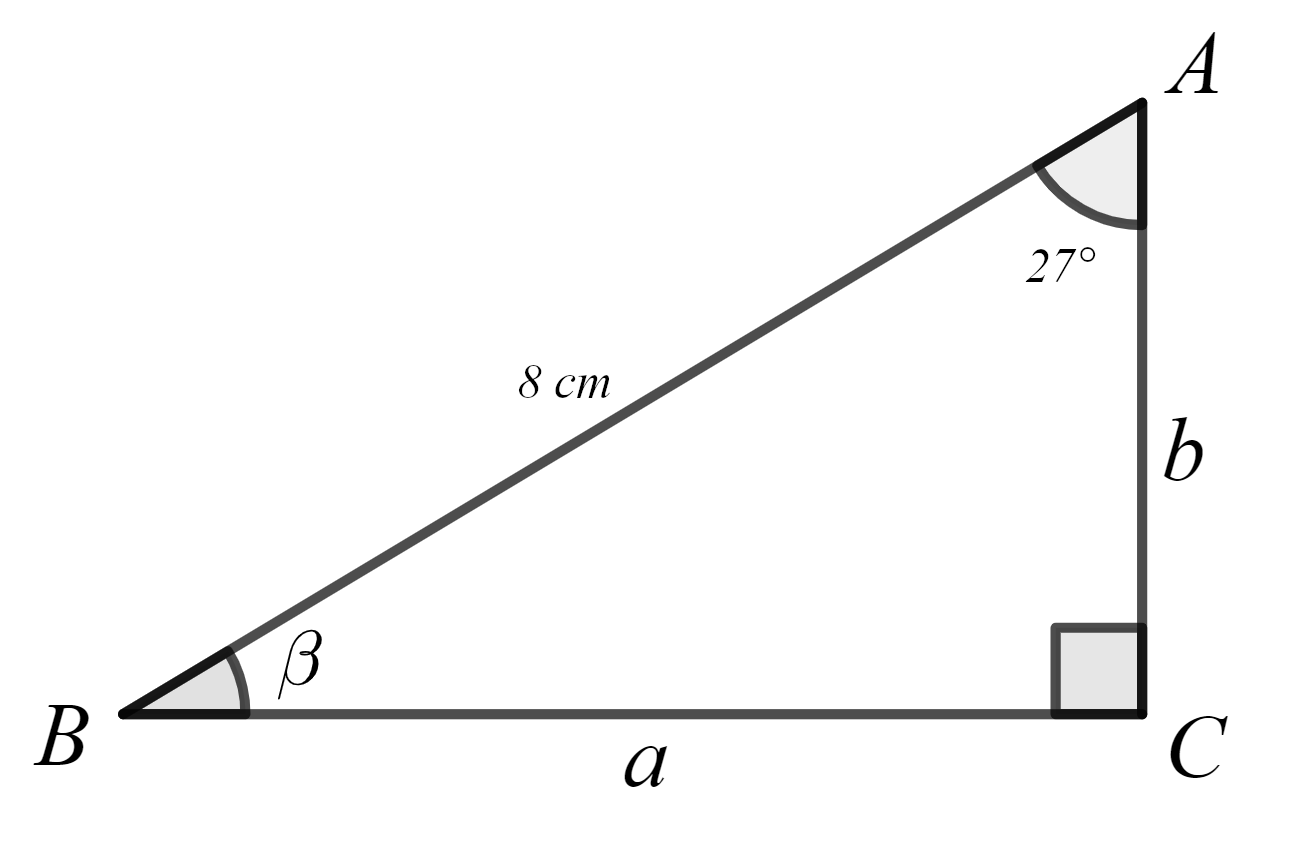
\includegraphics[width=0.3\textwidth]{images/trianglerectexemple.png}\\
$\beta=180-90-27=63^{\circ}$\\
En utilisant la trigonométrie:\\
$\sin(\alpha)=\dfrac{\text{opp}}{\text{hyp}} \Rightarrow \sin(27^{\circ})=\dfrac{\overline{BC}}{8}$\\
$\Rightarrow \overline{BC}=8 \cdot \sin(27^{\circ})=3.63\,cm$\\
$\cos(\alpha)=\dfrac{\text{adj}}{\text{hyp}} \Rightarrow \cos(27^{\circ})=\dfrac{\overline{AC}}{8}$\\
$\Rightarrow \overline{AC}=8 \cdot \cos(27^{\circ})=7.13\,cm$\\
\end{solution}

Il est tout à fait possible d’ajouter du code exécutable dans les solutions.


\end{document}
